\documentclass[12pt]{article}
\author{Lawrence Liu, UID: 405749034}
\usepackage{subcaption}
\usepackage{graphicx}
\usepackage{amsmath}
\usepackage{pdfpages}
\newcommand{\Laplace}{\mathscr{L}}
\setlength{\parskip}{\baselineskip}%
\setlength{\parindent}{0pt}%
\usepackage{xcolor}
\usepackage{listings}
\definecolor{backcolour}{rgb}{0.95,0.95,0.92}
\usepackage{amssymb}
\usepackage{empheq}

\newcommand*\widefbox[1]{\fbox{\hspace{2em}#1\hspace{2em}}}
\lstdefinestyle{mystyle}{
    backgroundcolor=\color{backcolour}}
\lstset{style=mystyle}
\title{Chem 20A Midterm 1}
\begin{document}
\maketitle
\section*{Problem 1}
\subsection*{(a)}
The bright lines are the photons emitted 
by the electrons as they fall back to a lower 
energy state.\\
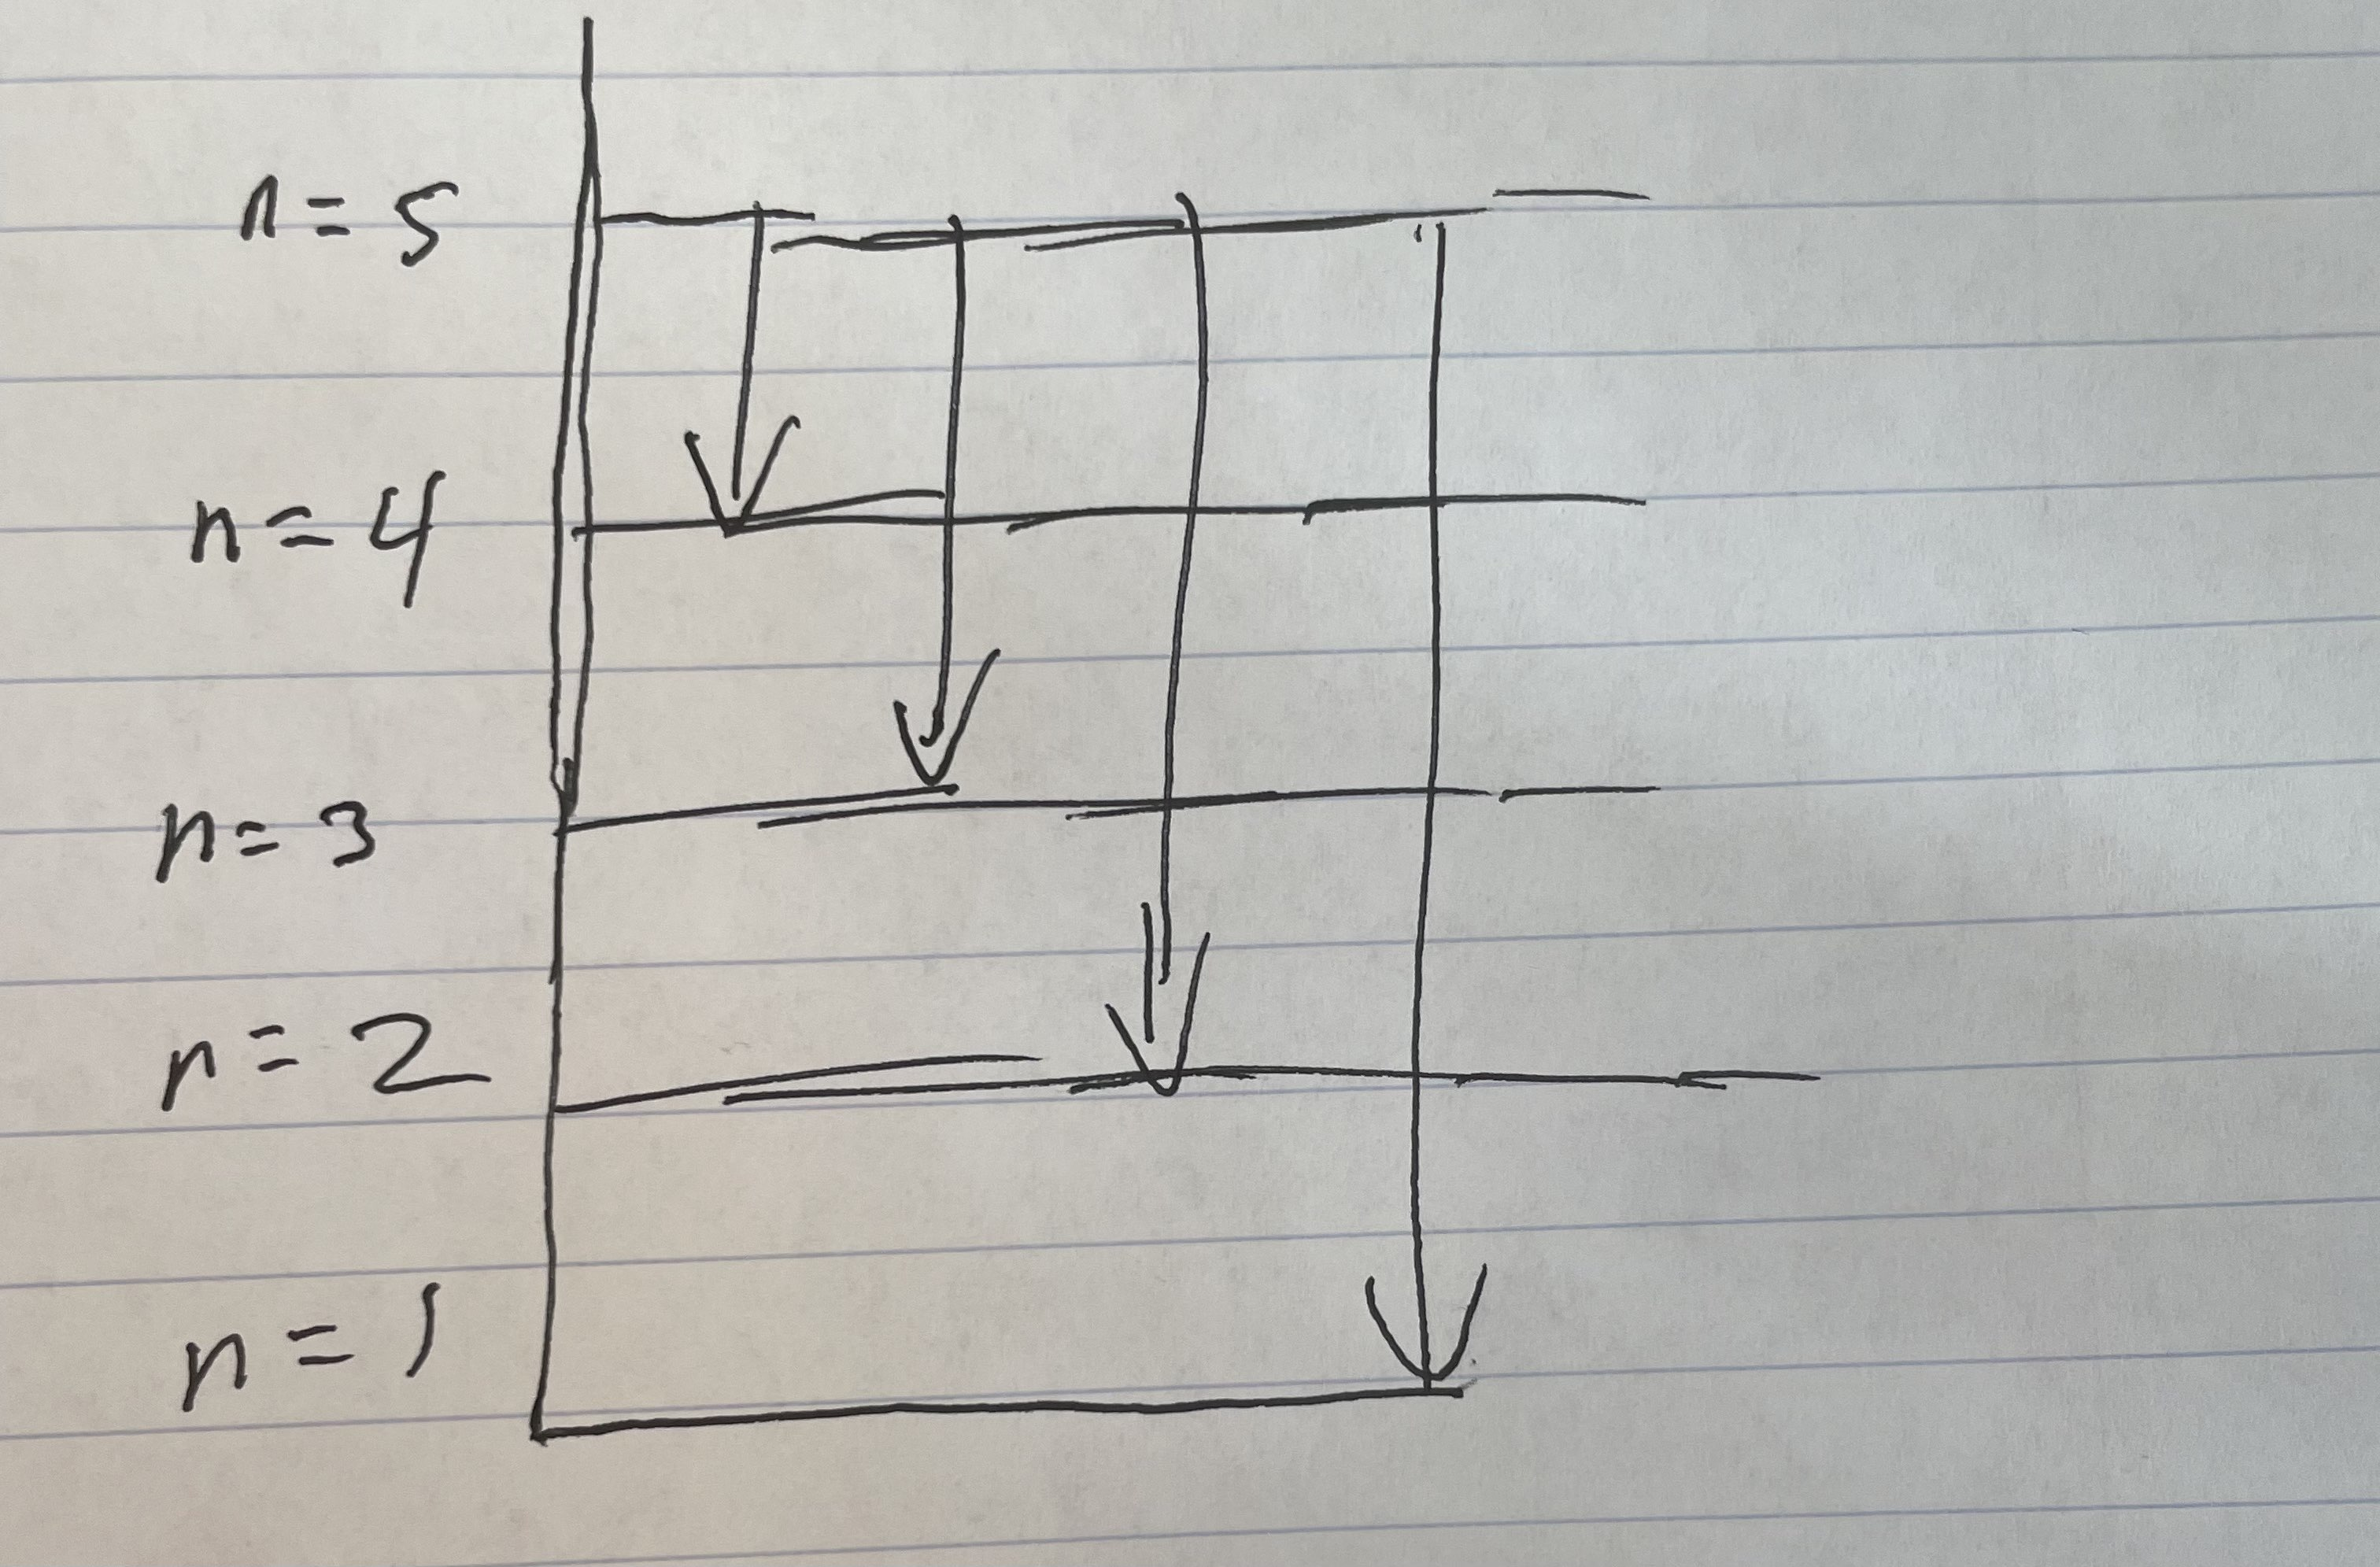
\includegraphics[
width=0.5\textwidth
]{1a.png}\\
Thus we would expect 4 lines.\\
\subsection*{(b)}
The lowest wavelength must corresponded to the highest energy
the 4th excited state ($n=5$) to the ground state ($n=1$). Thus the energy
of the emitted photon is
$$E=-\frac{Z^2}{5^2}-\left(-\frac{Z^2}{1^2}\right)$$
Since this is a lithium ion, $Z=3$. Thus we have that
$$E=3^2-\frac{3^2}{5^2}=7.92 \text{ rydbergs}$$
We have that the wavelength of the emitted photon is
$$\lambda=\frac{hc}{E}$$
$$\lambda=\boxed{11.505 nm}$$
\subsection*{(c)}
To remove the electron it will take 
$$E=\frac{Z^2}{n^2}$$
$$E=\frac{3^2}{3^2}=1 \text{ rydbergs}$$
$$E=\boxed{2.179\cdot10^{-18}J}$$
The wavelength of the light is 
$$\lambda=\frac{hc}{E}$$
$$\lambda=91.126nm$$
This falls in the ultraviolet region of the spectrum.
\section*{Problem 2}
\subsection*{(a)}
From periodic table, 
X is CL, so its atomic number is 17. Fluorine 
has an atomic number of 9, thus the atomic number of 
Y is 7.
\subsection*{(b)}
Let $C$ be the atomic weight 
of carbon, $H$ be the atomic weight of hydrogen,
$X$ be the atomic weight of chlorine, and $Y$ be the atomic weight of
Nitrogen, $O$ be the atomic weight 
of oxygen, and $Ru$ be the atomic weight of Ruthenium.
Thus the molecular weight is:
$$29\cdot C+33\cdot H+2\cdot X+2\cdot Y+ O+Ru$$
$$29\cdot 12.011+33\cdot 1.008+2\cdot 35.453+2\cdot 14.007+15.99+101.07= \boxed{597.566 g/\text{mol}}$$
\subsection*{(c)}
There must be the same number of protons in each isotope. Furthermore, 
since Ru's atomic number is 44, we know that there are 44 protons in
each isotope. Thus the number of neutrons in each isotope is:\\
99: 55 neutrons, 44 protons\\
100: 56 neutrons, 44 protons\\
101: 57 neutrons, 44 protons\\
102: 58 neutrons, 44 protons\\
104: 60 neutrons, 44 protons\\
\subsection*{(d)}
We have the density is g per L is $861g/L$. We have that 
a spherical solvent box with radius $100\AA$ has volume:
$$V=\frac{4}{3}\pi (100\AA)^3=4.188\cdot10^{-21}L$$
Thus the weight of the sphere is $3.606\cdot10^{-18}g$. 
We have that molar mass of Xylene is $106.16 g/mol$. 
Thus the number of molecules is: $20458.875$.
\section*{Problem 3}
\subsection*{(a)}
Because the energy of the laser is $\frac{hc}{600nm}=2.066eV$, 
which is less than the work function of $5.30eV$.
\subsection*{(b)}
We want the energy of the photon $\frac{hc}{\lambda}$ to be 
greater than the work function. We have that
$$\frac{hc}{\lambda}>5.30eV$$
$$\lambda<\frac{hc}{5.30eV}$$
$$\lambda<\boxed{233.932nm}$$
\subsection*{(c)}
The energy of the ejected photon is 
$$E=\frac{hc}{160nm}-5.30eV=2.449eV$$
We have that 
$$\lambda=\frac{h}{p}=\frac{h}{\sqrt{2m_e E}}= 0.783nm$$
\section*{Problem 4}
\subsection*{(a)}
Because it must be a standing wave, we must have that
$\psi(0)=\psi(4L)=0$. Thus we have that the wave function is
$$\psi(x)=\begin{cases}
    A\sin\left(kx\right) & \text{if } 0\leq x\leq 4L\\
    0 & \text{otherwise}
\end{cases}$$.
Since $\psi(4L)=0$, we have that $4kL=\pi n$ for 
$n=1,2,3,\ldots$. Thus we have that $k=\frac{n\pi}{4L}$.
\subsection*{(b)}
We have that 
$$H\psi(x)=E\psi(x)$$
Thus in the region $0\leq x\leq 4L$ we have that
$$\frac{h^2}{8\pi^2m}Ak^2\sin(kx)+\pi A\sin(kx)=AE\sin(kx)$$
Dividing by $A\sin(kx)$ we get 
$$\frac{h^2}{8\pi^2m}k^2+\pi=E$$
$$E=\boxed{\frac{h^2n^2}{128L^2m}+\pi}$$
\subsection*{(c)}
We have that the wavefunction for the 4th excited state is 
given by 
$$\psi(x)=\begin{cases}
    A\sin\left(\frac{5\pi}{4L}x\right) & \text{if } 0\leq x\leq 4L\\
    0 & \text{otherwise}
\end{cases}$$
Thus we have that the probability
of finding the electron in the region $L\leq x\leq 2L$ is
$$\int_{L}^{2L}|\psi(x)|dx=\int_{L}^{2L}A^2\sin^2\left(\frac{5\pi}{4L}x\right)dx$$
\section*{Problem 5}
\subsection*{(a)}
We have the following quantum number combinations for $n=3$
We have the 3s orbital:
$$n=3, l=0, m_l=0$$
We have the 3p orbitals:
$$n=3, l=1, m_l=-1$$
$$n=3, l=1, m_l=0$$
$$n=3, l=1, m_l=1$$
We have the 3d orbitals:
$$n=3, l=2, m_l=-2$$
$$n=3, l=2, m_l=-1$$
$$n=3, l=2, m_l=0$$
$$n=3, l=2, m_l=1$$
$$n=3, l=2, m_l=2$$
\subsection*{(b)}
Because we must have $|m_l|\leq l$ and $m_l$ be an integer. And thus for the 
3p orbitals we have 3 possible values for $m_l$, (-1,0,1).
Likewise for the 3d orbitals we have 5 possible values for $m_l$, 
(-2,-1,0,1,2). Thus we have that there are 3 
3p orbitals and 5 3d orbitals.
\subsection*{(c)}
In order to have 0 probability, 
we must have that $R_{4p}(r=0)$. Thus we must have that 
$$\frac{2Zr}{n}\left(20-10\frac{2Zr}{n}+\frac{4Z^2r^2}{n^2}\right)=0$$
Thus this can happen when $r=0$, or when 
$$\left(20-10\frac{2Zr}{n}+\frac{4Z^2r^2}{n^2}\right)=0$$
This can only happen when $\frac{2Zr}{n}=\frac{10\pm\sqrt{100-80}}{2}$.
$\frac{10+\sqrt{100-80}}{2}=7.236$, and 
$\frac{10-\sqrt{100-80}}{2}=2.764$. Thus we have that the corresponding 
$r$ is $7.326\frac{n}{2Z}=\frac{7.326\cdot 4}{2\cdot 4}=3.618a_0$ and
and $2.674\frac{n}{2Z}=\frac{2.674\cdot 4}{2\cdot 4}=1.381a_0$
Therefore the distances where we would expect 
$R_{4p}(r=0)$ are $r=0,1.914\cdot10^{-10}m, 7.313\cdot10^{-11}m$.
\subsection*{(d)}
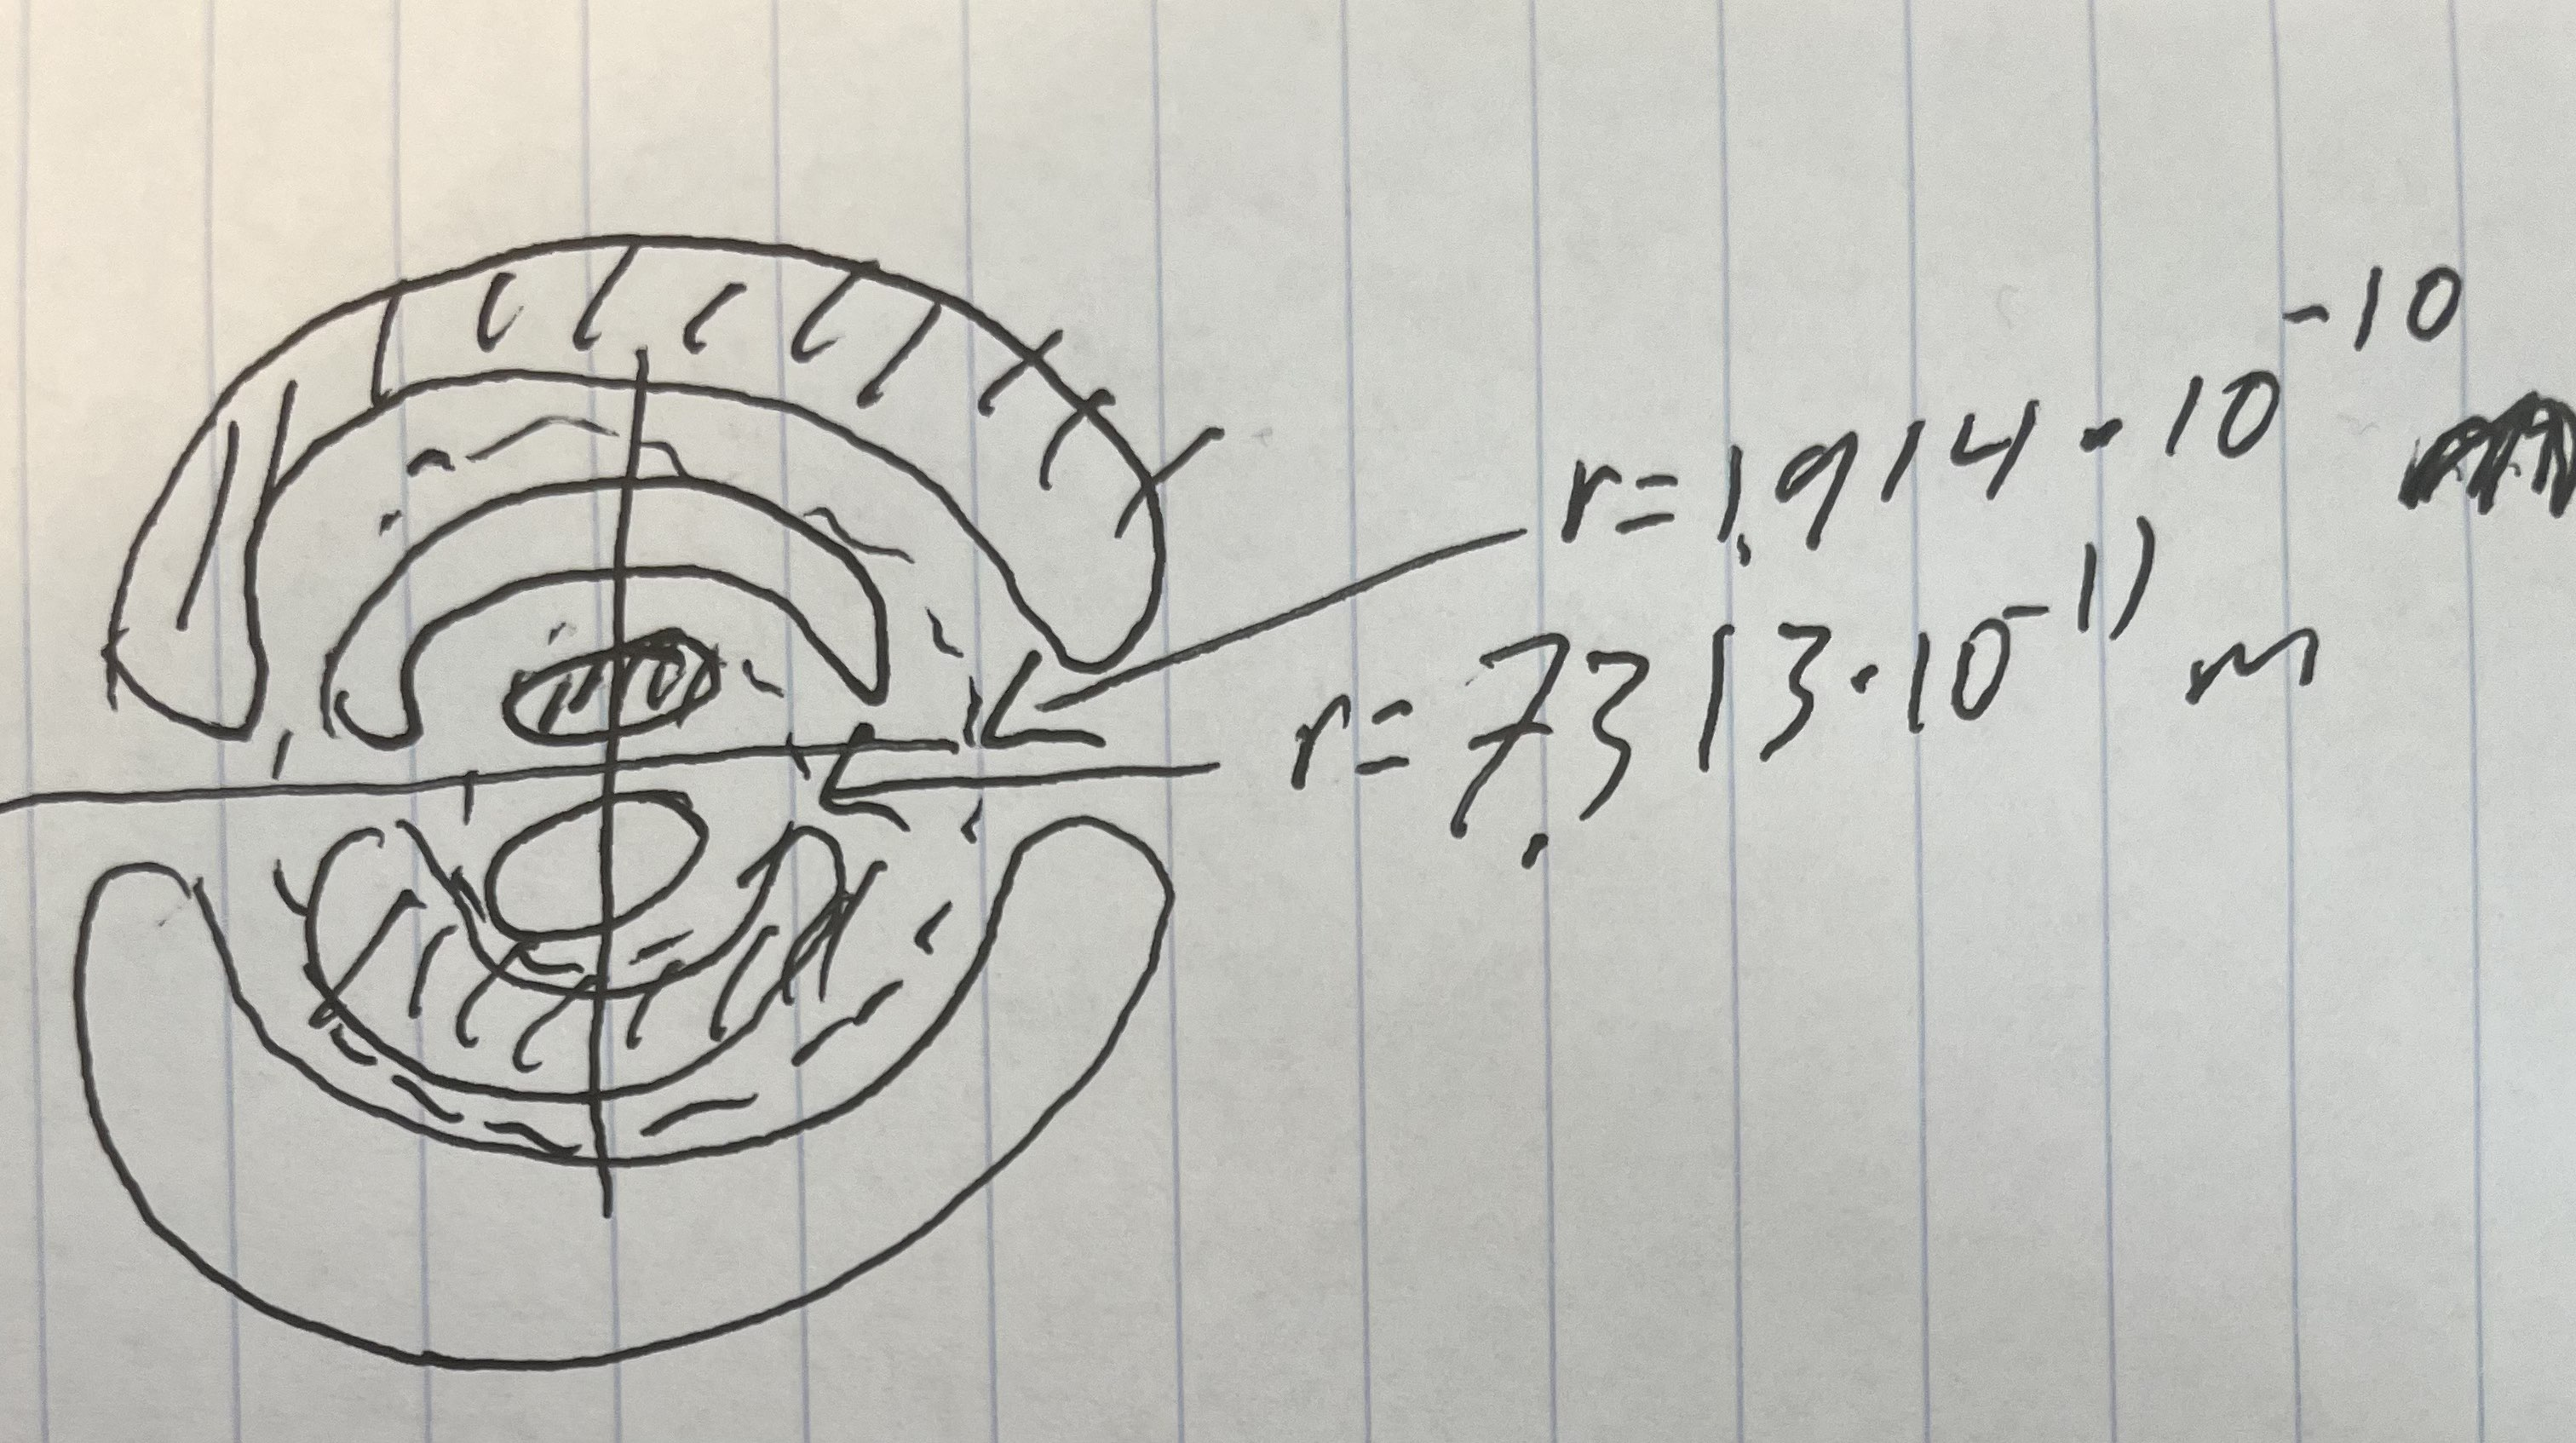
\includegraphics[width=0.5\textwidth]{5d.png}


\end{document}
